We will now calculat the mismatch for a fully-coherent search given the
random walk in phase, frequency, and spin-down rate defined in the previous
section.

Let us begin by expanding the metric-mismatch summation from Eqn.~\eqref{eqn:
mismatch}.  Writing the summations explicitly, we have
\begin{align}
m & = g_{\alpha\beta i j}\dl^{\alpha i}\dl^{\beta j}  \\
&=\s{i=1}{N}\s{j=1}{N}g_{\alpha\beta i j}\dl^{\alpha i}\dl^{\beta j}  \\
&= \s{i=1}{N}g_{\alpha\beta i i}\dl^{\alpha i}\dl^{\beta i}
+ \s{i=1}{N} \s{\substack{j=1\\ j \ne i}}{N} g_{\alpha \beta ij}\dl^{\alpha i}\dl^{\beta j}.
\end{align}
The summation has been intentionally split into terms for which the two
segments are the same and those for which they are different. The metric when
the reference time is at the beginning of each segment is given by equation
\eqref{eqn: metric equal segments tref 0}. By considering the metric for the
two cases, we can write the two distinct components as
\begin{equation}
g_{\alpha\beta ij} = \left\{
\begin{array}{cc}
g_{\alpha\beta}^{\mathrm{E}} & \textrm{ if } i =j \\
g_{\alpha\beta}^{\mathrm{NE}} & \textrm{ if } i  \ne j
\end{array}\right.  .
\end{equation}
Then the mismatch can be calculated from
\begin{align}
m &= \s{i=1}{N}g_{\alpha\beta}^{\mathrm{E}}\dl^{\alpha i}\dl^{\beta i}
+ 2\s{i=1}{N} \s{j=1}{i-1} g_{\alpha \beta}^{\mathrm{NE}}\dl^{\alpha i}\dl^{\beta j} .
\label{eqn: mismatch sep}
\end{align}

\subsection{Writing the parameter offsets in terms of normal distributions}
Equations~\eqref{eqn: f offset} and \eqref{eqn: phi
offset} give the offsets as functions of the offsets in higher order
parameters. In order to calculate statistical values, we now write these in terms of
the normal distributions from which the random walks are constructed.
Substituting Eqn.~\eqref{eqn: delta fdot n} into Eqn.~\eqref{eqn: f offset} and using the summation properties defined
in Appendix~\ref{sec: summation identities}, we have
\begin{align}
\Delta \f_{i}  & = \s{j=1}{i}\tn \f_{j}
+ \s{j=1}{i-1}\s{k=1}{j}\tn \fdot_{k} \dT ,  \\
& = \s{j=1}{i}\tn \f_{j}
+ \s{j=1}{i-1}(i-j)\tn \fdot_{j} \dT .
\label{eqn: delta f n}
\end{align}
Similarly, substituting this equation into Eqn.~\eqref{eqn: phi offset} we
have
\begin{align}
\begin{split}
\Delta\phi_{i} & = \s{j=1}{i}\tn \phi_{j}
+ 2\pi \left(\s{j=1}{i-1}\Delta\f_{j}\dT
+ \frac{1}{2}\s{j=1}{i-1}\Delta\fdot_{j}\dT^{2}\right) \\
& = \s{j=1}{i}\tn \phi_{j} + 2\pi\left(\s{j=1}{i-1}\left(\s{k=1}{j}\tn\f_{k}
+ \s{k=1}{j-1}(j-k)\tn\fdot_{k}\dT\right)\dT
 + \frac{1}{2}\s{j=1}{i-1}\s{k=1}{j}\Delta\fdot_{k}\dT^{2} \right)  \\
& = \s{j=1}{i}\tn \phi_{j} + 2\pi\left(\s{j=1}{i-1}(i-j)\tn\f_{j}\dT
 + \s{j=1}{i-1}\s{k=1}{j-1}(j-k)\tn\fdot_{k}\dT^{2}
 + \frac{1}{2}\s{j=1}{i-1}(i-j)\Delta\fdot_{j}\dT^{2} \right)  \\
& = \s{j=1}{i}\tn \phi_{j} + 2\pi\left(\s{j=1}{i-1}(i-j)\tn\f_{j}\dT
 + \frac{1}{2}\s{j=1}{i-1}\left(\left(i-j\right)\left(i-j-1)\right)
 + (i-j)\right)\tn\fdot_{j}\dT^{2}\right)  \\
& = \s{j=1}{i}\tn \phi_{j} + 2\pi\left(\s{j=1}{i-1}(i-j)\tn\f_{j}\dT
 + \frac{1}{2}\s{j=1}{i-1}(i-j)^{2}\tn\fdot_{j}\dT^{2}\right)
\end{split}
\label{eqn: delta phi n}
\end{align}

\subsection{Taking the expectation}

In Eqn.~\eqref{eqn: delta fdot n}, Eqn.~\eqref{eqn: delta f n},
Eqn.~\eqref{eqn: delta phi n} we have written the parameter space offsets
(which are to be used in calculating the mismatch) purely in terms of the
random walk distributions $\tn \phi_i$, $\tn \f_i$, and $\tn \fdot_i$. We can
calculate the mismatch exactly given a set of random walk jumps by inserting
these into Eqn.~\eqref{eqn: mismatch sep}. However, since we are dealing with
statistical quantities, we can instead infer the behaviour of the mismatch
under the random walk by taking an expectation.

Inseting Eqn.~\eqref{eqn: delta fdot n}, Eqn.~\eqref{eqn: delta f n},
Eqn.~\eqref{eqn: delta phi n}  in Eqn.~\eqref{eqn: mismatch sep} yields a
number of terms with all the permutations of two terms from $[\tn \phi, \tn \f,
\tn \fdot]$. Taking the expection, all the cross-correlated terms, such as
$\tn\phi_{i}\tn \fdot$, will have an expectation of zero since the steps of the
random walk are independent. The only non-vanishing terms are given by
\begin{align}
E[\tn\phi_{i}\tn\phi_{j}] &= \delta_{ij}\sigP, &
E[\tn\f_{i}\tn\f_{j}] &= \delta_{ij}\sigF,&
E[\tn\fdot_{i}\tn\fdot_{j}] &= \delta_{ij}\sigS,
\end{align}
After some simplification we find that the mismatch is given by
\begin{align}
\begin{split}
E[m]   = &  \frac{A_{\phi}}{6} \left(N - \frac{1}{N}\right)
+ \frac{\pi^{2} A_{{f}}}{30}\left(4 N^{3} + 5 N^{2} + \frac{1}{N}\right)\\
 & +  \frac{\pi^{2} A_{{\dot{f}}}}{3780} \left(66 N^{5} - 21 N^{3} + 105 N^{2}
 + 217 N + 63 - \frac{94}{N}\right),
\end{split}
\label{eqn: expectation}
\end{align}
where
\begin{equation}
	A_{\phi} = \sigP \;\;\;\;\;
    A_{\f} = \sigF\Delta T^{2} \;\;\;\;\;
    A_{\fdot} = \sigF\Delta T^{4},
\end{equation}
define three `activity parameters'.

\subsection{Verifying the results}
Recalling that $N=\Tobs/\Delta T$, Eqn.~\eqref{eqn: expectation} makes
predictions for the leading order
scaling of the three random walks with observation period
\begin{equation}
E[m]_{PN} \sim \sigP \Tobs, \hspace{10mm}
E[m]_{FN} \sim \sigF \Tobs^{3}, \hspace{10mm}
E[m]_{FN} \sim \sigS \Tobs^{5}.
\end{equation}

We can observe this behaviour directly and verify the predictions made by
Eqn.~\eqref{eqn: expectation} by comparing with exact numerical results. That
is, using the signal injection and recovery tools developed in Sec.~\ref{sec:
narrow-band method} of Chapter.~\ref{sec: timing noise in cgw} we simulate
signals undergoing a random walk and calculate the corresponding mismatch (no
minimisation step is done here, this is discussed in the next section). In
particular, we perform three Monte Carlo studies for a random walk in the
phase, frequency, and spin-down rate and in each case compre the simulated
results with the analytic prediction. The results are shown in Fig.~\ref{fig: rw I}
and demonstrate good agreement between the simulation means and the prediction
of Eqn.~\eqref{eqn: expectation}.

\begin{figure}[ht]
\centering
\subfloat[Random walk in phase]{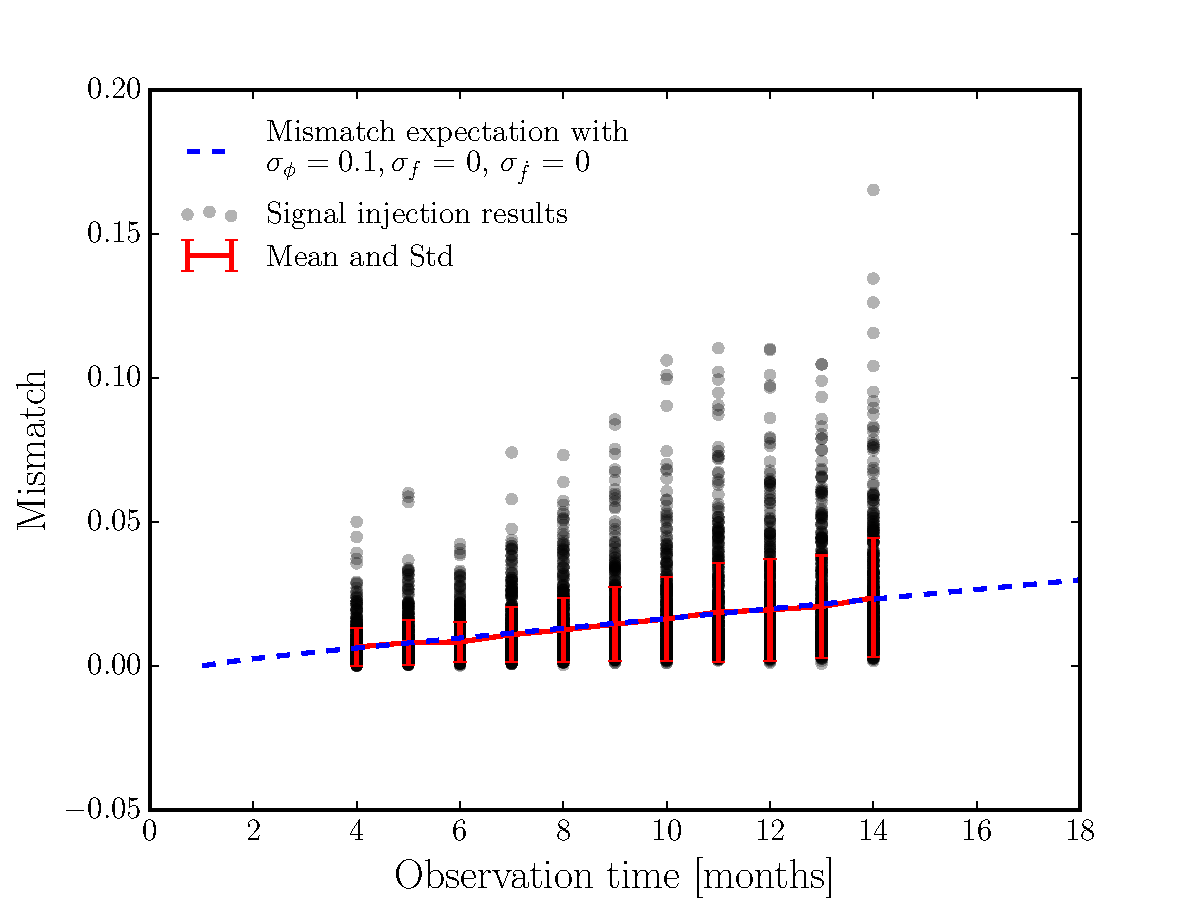
\includegraphics[width=0.5\textwidth]{ExpectationPhase}}
\subfloat[Random walk in frequency]{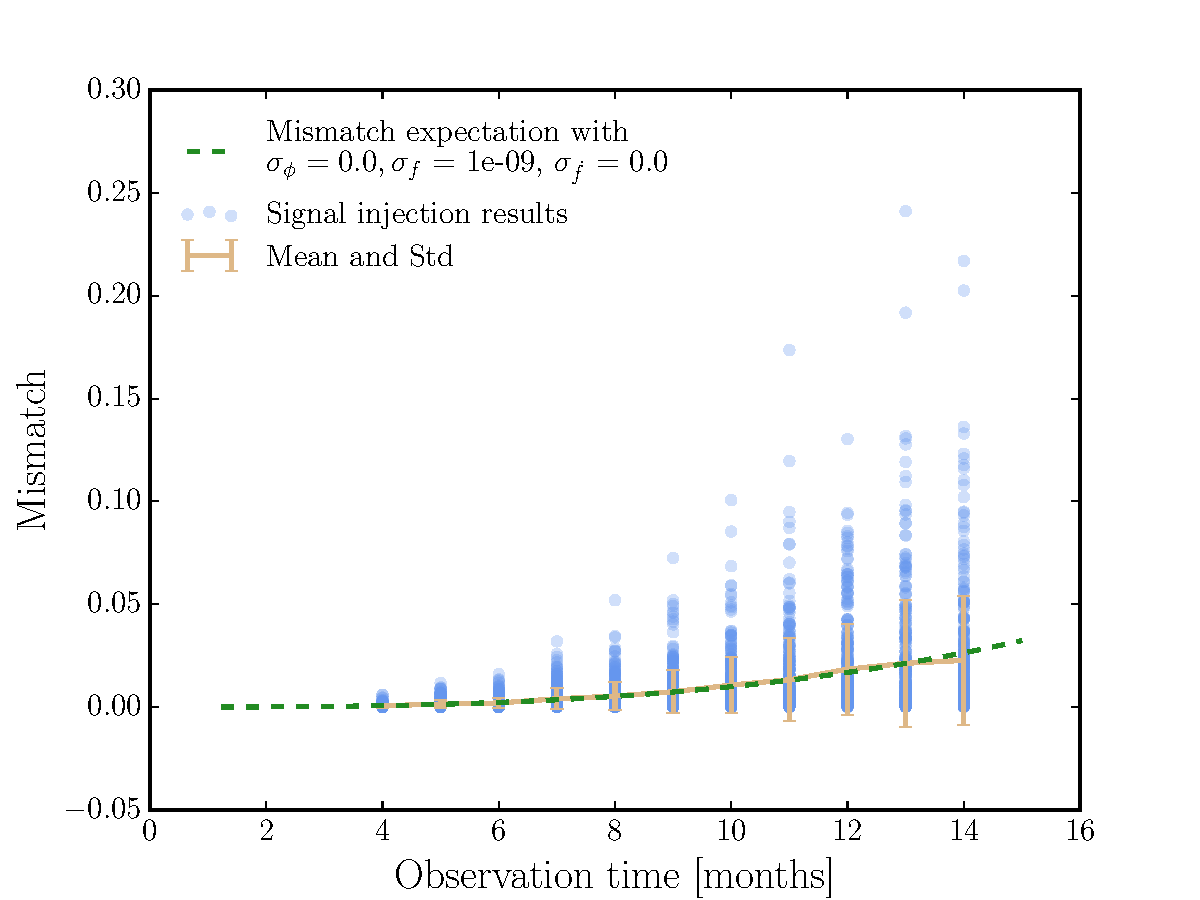
\includegraphics[width=0.5\textwidth]{ExpectationFrequency}}\\ \subfloat[Random walk in spin-down]{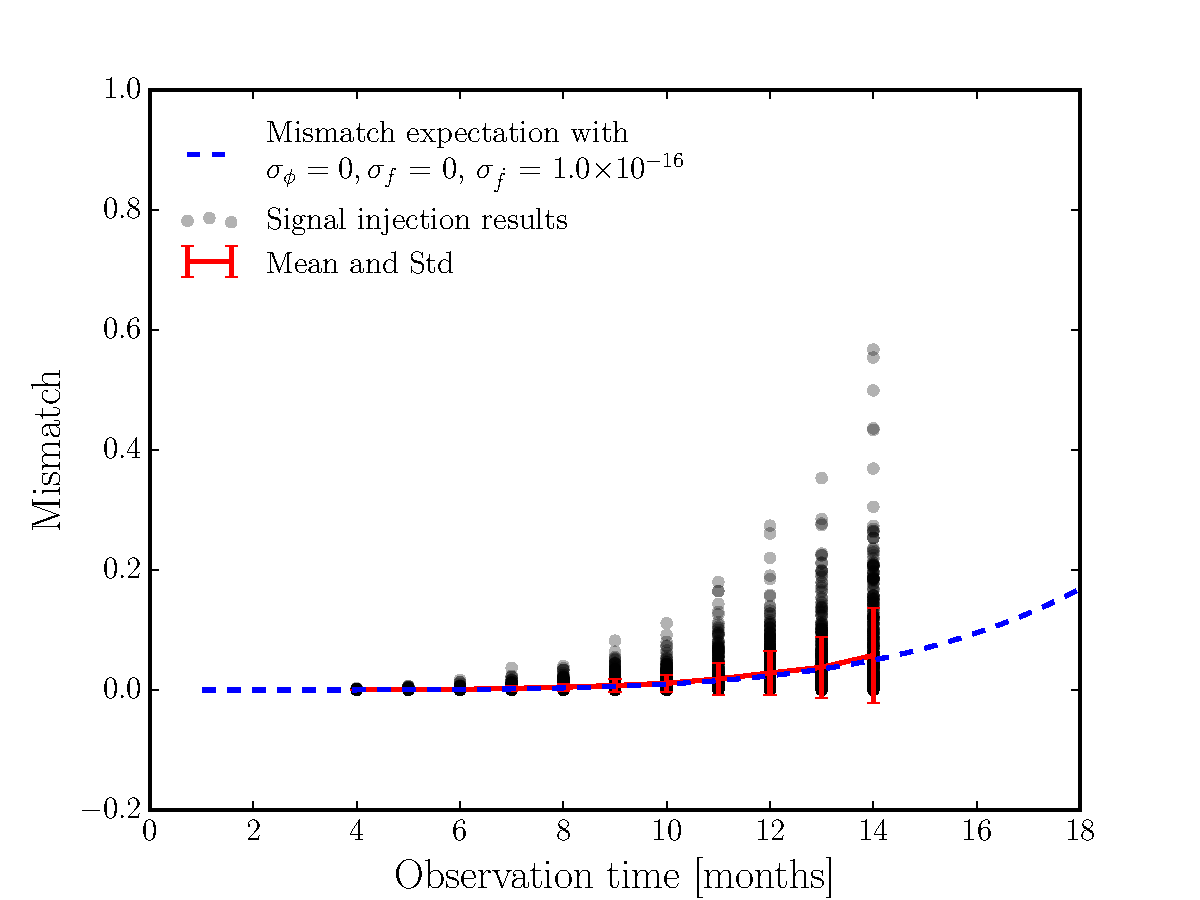
\includegraphics[width=0.5\textwidth]{ExpectationSpindown}}
\caption{A comparison of Monte Carlo numerical simulated mismatch with the prediction
of Eqn.~\eqref{eqn: expectation} for a random walk in the phase, frequency,
and spin-down rate.}
\label{fig: rw I}
\end{figure}

\subsection{Implied scaling}

Eqn.~\eqref{eqn: expectation} predicts the variation in mismatch with
observation time due to a random walk in the parameters of the signal. The
random walk occurs at fixed intervals of $\dT$ and in three parameters, as such
the mismatch is a function of all these variables. This method differs from
results in the literature studying timing noise \citep{Cordes1981} where the
steps are Poisson distributed in time with an average rate. The choice of a
fixed $\dT$ is necceciated by the ease of calculation for regular intervals,
but is consisent with the description of timing noise provided by the Crab
ephemeris in Sec.~\ref{sec: timing noise in cgw}.  For the expectation of the
mismatch to be physical, we should expect that, at least to leading order, it
is invariant to a suitable combination of $\dT$ and $\sigma$. Equivalently we
imagine that if the Crab ephemeris was updated every half a month instead of
once a month, we should measure the same mismatch for the same observation
period.

To leading order, for the expected mismatch to be invariant to changes in $\dT$
we require
\begin{equation}
\sigP \sim \dT \;\;\;\;\; \sigF \sim \dT \;\;\;\;\; \sigS \sim \dT
\end{equation}
Importantly this result agrees with the description of a Compound Poisson
process in the limit where the many events occur during the observation period
$\dT$.
\meta{Greg: not sure about this claim}
